\chapter{Metodologia}
\section{Caracterização do Objeto de Estudo}\label{sec:carac}
O objeto de estudo deste projeto é o design preliminar do motor-foguete de propelente líquido alimentado com \gls{EthaLOx}, desenvolvido para fins acadêmicos e experimentais. Trata-se de um sistema de propulsão de pequeno porte, com empuxo médio estimado de 1 kN, concebido como base para pesquisa e desenvolvimento de tecnologias aplicadas a motores-foguete. O projeto está sendo conduzido por estudantes da \Gls{UFSC} com o objetivo de consolidar conhecimento técnico nas áreas de injeção, resfriamento, alimentação de propelentes, controle e desempenho térmico-estrutural.

O motor será operado em ciclo \gls{EPFS}, buscando simplicidade de implementação e controle, além de maior compatibilidade com estudos acadêmicos de laboratório. A escolha dos propelentes baseia-se em critérios de disponibilidade, propriedades termoquímicas e maturidade tecnológica, sendo o etanol adotado como combustível e o oxigênio líquido como oxidante.

O objeto de estudo é abordado exclusivamente em nível teórico e analítico, com foco na definição de parâmetros de projeto, critérios de dimensionamento e integração dos subsistemas. As soluções técnicas estudadas consideram a aplicação de manufatura aditiva, ou \gls{AM}, metálica, superfícies de transferência de calor otimizadas, injetores com geometrias compatíveis com \gls{AM} e válvulas criogênicas compactas. A ênfase está na avaliação do comportamento funcional de cada subsistema dentro de um cenário teórico de operação, sem execução de testes físicos nem produção de protótipos nesta etapa.

O estudo do motor-foguete como objeto central permite a investigação coordenada de múltiplos aspectos da engenharia aeroespacial, incluindo transferência de calor em canais regenerativos, desempenho de bombas e impulsores, estabilidade de combustão, escolha de materiais e integração térmica de componentes submetidos a altos gradientes de temperatura e pressão.

\section{Universo de Pesquisa}\label{sec:univ}
A pesquisa concentra-se no desenvolvimento de soluções técnicas aplicáveis a motores de pequeno porte voltados à propulsão experimental, sem aplicação direta em sistemas comerciais ou operacionais previstas inicialmente, mas com conceitos e tecnologia que podem ser escalados a demais projetos. As atividades serão conduzidas por meio de levantamento bibliográfico, modelagem teórica e análise de viabilidade de subsistemas, sem realização de testes físicos ou experimentação prática, mas sim por meio de estudos conceituais e simulações de fenômenos e design a serem analisados.

\section{Estudos Propostos}\label{sec:estudos}
O projeto \Gls{RAPID} encontra-se em fase inicial, com foco na definição de pré-requisitos técnicos e no desenvolvimento conceitual dos principais subsistemas de um motor-foguete de propelente líquido, com empuxo médio estimado de 1 kN, utilizando etanol e oxigênio líquido como propelentes. Esta etapa visa estabelecer a base teórica e os parâmetros de projeto necessários para o avanço das atividades de desenvolvimento.

\section{Abordagem de Gerenciamento de Equipe}\label{sec:geren}
A gestão do trabalho entre os membros do projeto \Gls{RAPID} será conduzida com base na metodologia ágil, utilizando o \textit{framework} Scrum como modelo organizacional. A estrutura de Scrum adotada prevê ciclos quinzenais, com duração de quinze dias, coincidentes com as etapas previstas no Cronograma Físico (Anexo~\ref{cronograma}) do projeto e na subdivisão apresentada na seção \ref{sec:fases}. Essa sincronização permite que a organização do trabalho individual e coletivo esteja diretamente vinculada às entregas esperadas em cada fase do projeto.

O Scrum é um modelo de gestão ágil iterativo e incremental, originalmente desenvolvido para projetos de software, mas amplamente adotado em ambientes de engenharia e pesquisa. Ele estabelece papéis claros, rituais periódicos e priorização contínua de tarefas~\cite{Bott2020}. No contexto do projeto \Gls{RAPID}, cada ciclo, de duração quinzenal, inclui a definição de tarefas a serem desenvolvidas, a revisão de entregas anteriores e a reavaliação de prioridades com base nas dependências técnicas e nas metas de desenvolvimento. O foco está na flexibilidade, no acompanhamento contínuo e na divisão eficiente do trabalho entre os membros da equipe.

A organização das tarefas será feita por meio de um sistema visual de kanban, utilizando a plataforma gratuita \textit{Deck}, que centraliza a gestão de tarefas individuais e coletivas. O \textit{Deck} está integrado a um servidor privado que reúne a infraestrutura digital da equipe, incluindo documentação técnica, bibliografia de referência, controle de versões, organização de arquivos, registros de reuniões e acompanhamento do progresso. Esse sistema garante rastreabilidade, consistência e facilidade de acesso às informações por todos os integrantes, mesmo em atividades assíncronas.

A abordagem de gerenciamento de equipe está estruturada para garantir autonomia operacional, priorização clara de atividades e capacidade de adaptação contínua, respeitando as características de um ambiente de pesquisa e projeto. A organização individual do trabalho está vinculada à execução das tarefas técnicas previstas na secção \ref{sec:metod}, que detalha a lógica de desenvolvimento adotada no \Gls{RAPID}.

\section{Abordagem Metodológica do Projeto}\label{sec:metod}

A condução metodológica do projeto \Gls{RAPID} é baseada no modelo de gerenciamento de tecnologia da NASA, o NPR 7120.8A \cite{NASAResearchTechnology2018}, adaptado para o contexto acadêmico de desenvolvimento de um sistema de propulsão líquido de pequeno porte. O ciclo de desenvolvimento adotado segue uma abordagem iterativa e evolutiva, típica de processos de engenharia de design, priorizando flexibilidade, refinamento progressivo e validação conceitual.

\begin{figure}[h!]
    \centering
    \caption{Mapa do processo de pesquisa de design preliminar adotado no projeto \Gls{RAPID}.}
    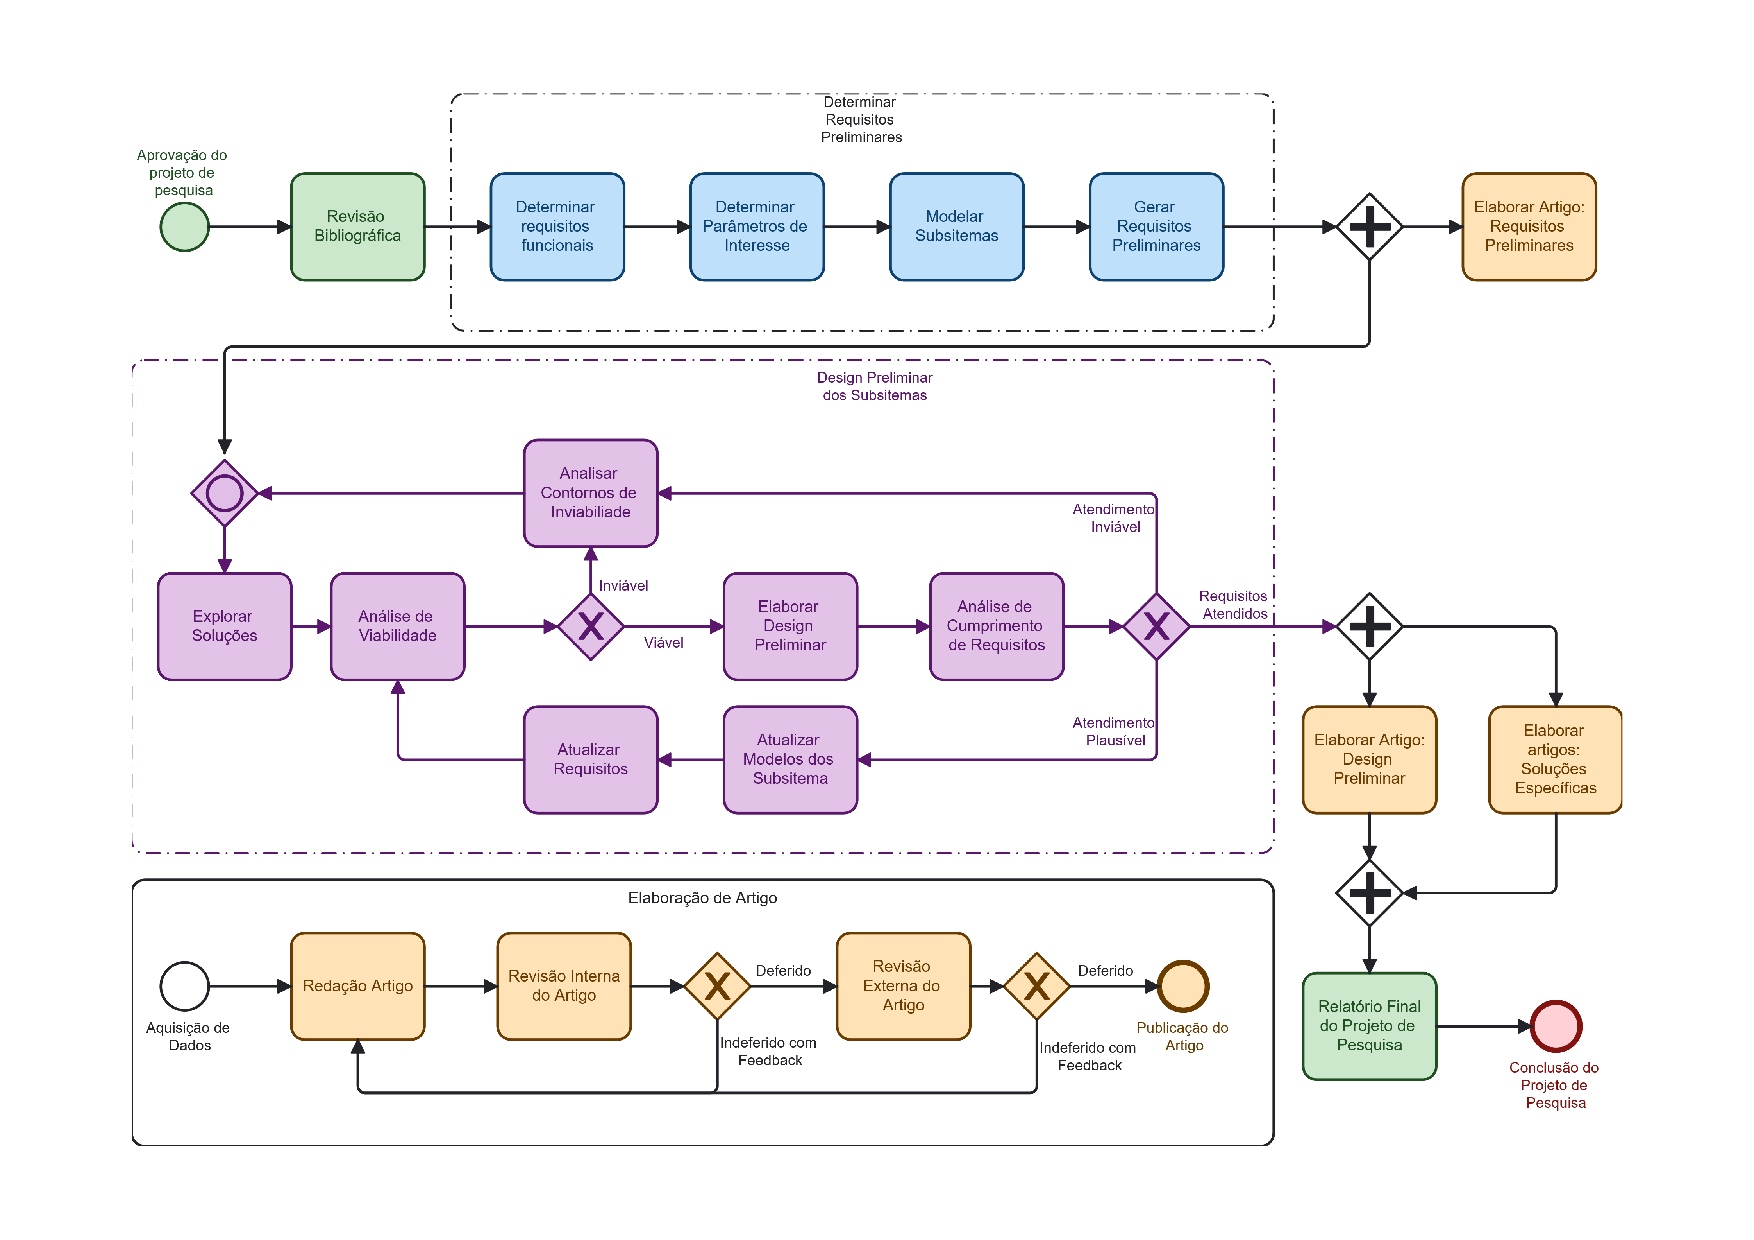
\includegraphics[width=0.85\textwidth]{Imagens/ProcessoDePesquisaDeDesign}
    \fonte{Elaborado pelo Autor (2025).}
    \label{fig:bpmn}
\end{figure}

O processo metodológico é representado na Figura~\ref{fig:bpmn}, que ilustra o ciclo de pesquisa em design adotado no projeto. Esse ciclo compreende iterações sucessivas entre as atividades de modelagem, análise, proposição de soluções e revisão. Isso permite uma adaptação contínua das soluções técnicas em função dos requisitos, restrições e novas descobertas.

Além disso, o projeto adota uma abordagem de desenvolvimento baseada em modelos, conhecida como \Gls{MBSE}. Essa abordagem permite que modelos matemáticos e computacionais sirvam como elementos centrais na definição, análise e validação do sistema como um todo. O uso do \Gls{MBSE} contribui para maior rastreabilidade, consistência entre requisitos e soluções e suporte à tomada de decisão durante as fases de projeto \cite{EstefanMBSE2008}.

\begin{figure}[h!]
    \centering
    \caption{Exemplo de diagrama esquemático de performance de um motor \gls{EPFS} otimizado com \gls{RoCAT}.}
    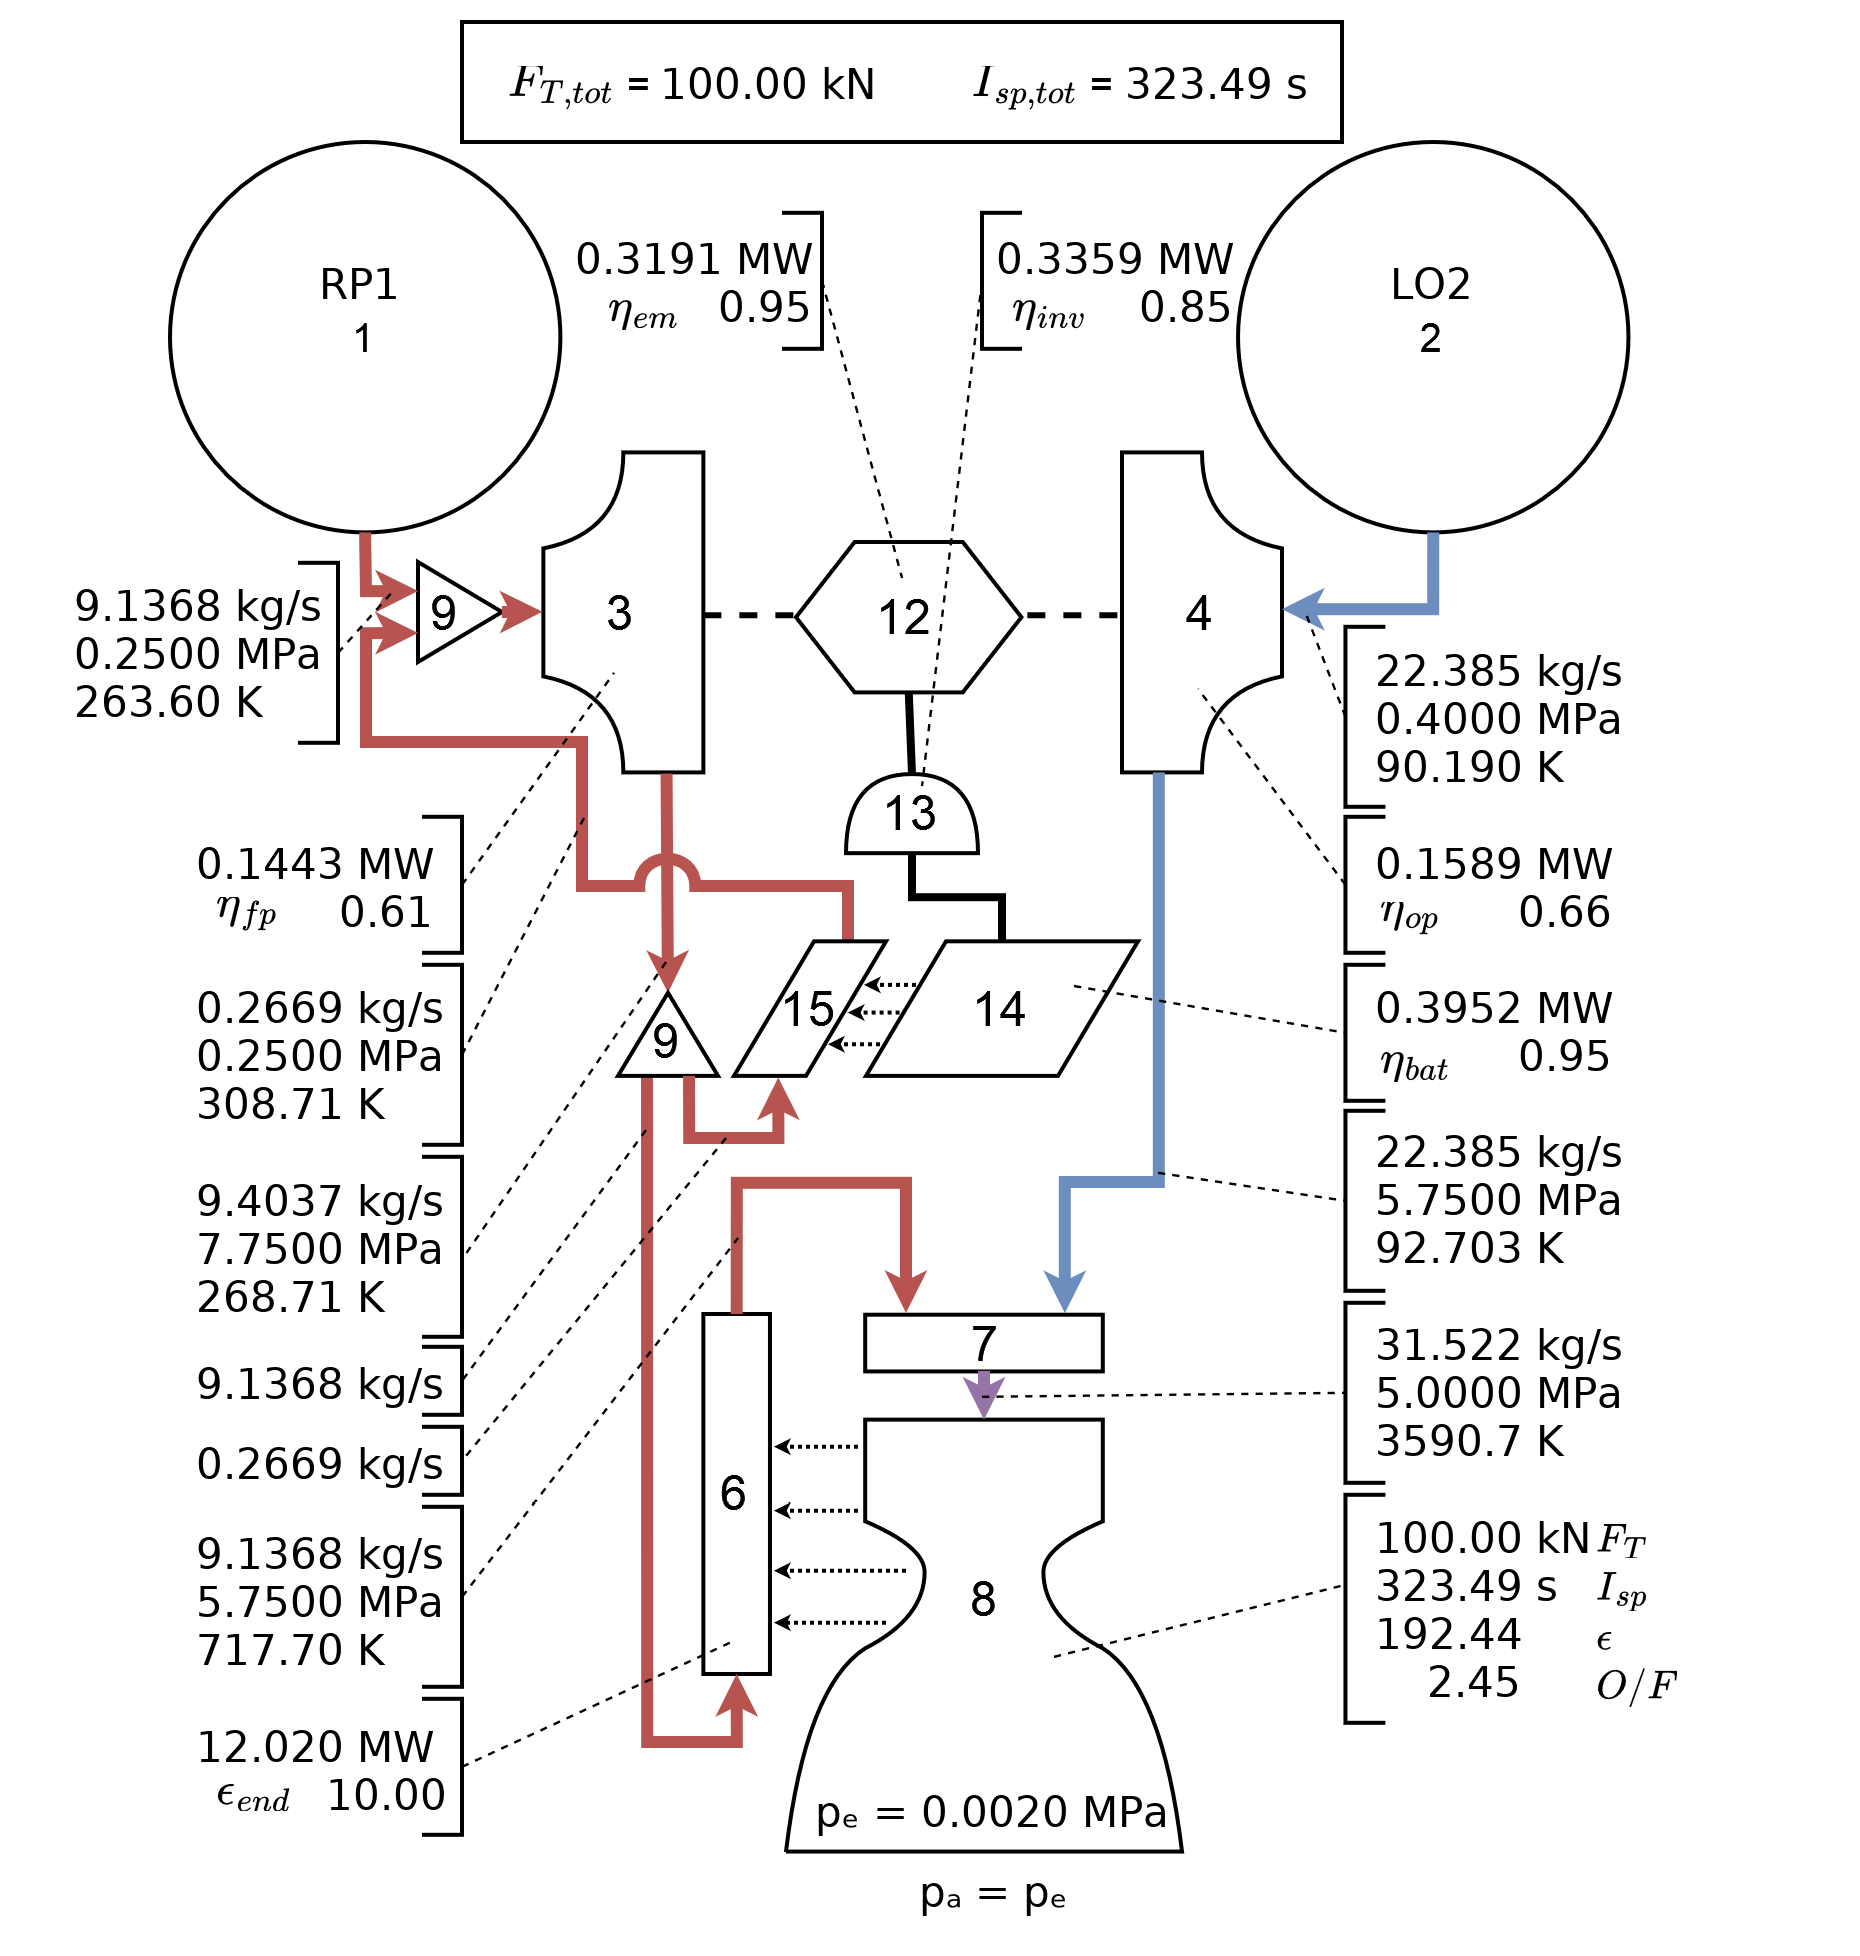
\includegraphics[width=0.85\textwidth]{Imagens/EPFS.png}
    \fonte{\textcite{Berg2023}}
    \label{fig:EPFS}
\end{figure}

No caso específico do \Gls{RAPID}, será desenvolvido um modelo matemático do sistema de propulsão, com foco no ciclo \gls{EPFS} e em sua interação com os subsistemas de alimentação, combustão e resfriamento. Um exemplo de representação funcional desse modelo pode ser visto na Figura~\ref{fig:EPFS}, onde se observa a lógica de operação e os parâmetros envolvidos na otimização de performance com a ferramenta \gls{RoCAT}.

As fases de projeto estão organizadas de modo a permitir adaptação dinâmica dos objetivos técnicos conforme os resultados obtidos em cada iteração. Essa estrutura favorece a aprendizagem contínua, a integração progressiva dos subsistemas e o amadurecimento gradual da solução até o design preliminar consolidado.

\section{Decomposição do Trabalho}\label{sec:trabalho}
O plano de trabalho, representado no cronograma apresentado no Anexo~\ref{cronograma}, está estruturado em três fases lógicas e interdependentes, permitindo a condução sequencial e controlada das atividades. Essa segmentação viabiliza a definição de marcos intermediários e a entrega de resultados concretos em cada etapa, alinhando-se a boas práticas de gerenciamento de projetos.

Cada fase foi subdividida em sub-fases específicas, cuja conclusão está associada a marcos técnicos internos que têm por objetivo revisar o progresso, validar os requisitos definidos e orientar ajustes no escopo técnico conforme necessário.

No contexto da abordagem metodológica do projeto, os marcos técnicos estarão associados a análises formais de progresso, validação de soluções desenvolvidas e consolidação de decisões técnicas. Esses marcos têm como objetivo orientar o refinamento do projeto, registrar o estado de maturidade técnica e fundamentar a produção de documentos ou estudos que sustentem as próximas etapas do desenvolvimento.


\section{Estrutura de Fases}\label{sec:fases}

Antes do início das fases, foi definido um período equivalente a dois ciclos de Scrum, reservado exclusivamente para a revisão bibliográfica dos temas listados para pesquisa. A partir dessa revisão e da sistematização das informações pelos membros da equipe, foram estabelecidos os fundamentos técnicos que orientam a organização do projeto. Com base nisso, as fases foram iniciadas e seguem a seguinte estrutura:

\subsection{Fase I: Revisão Bibliográfica}
Essa etapa tem como foco a fundamentação técnica e a definição dos temas específicos de estudo. Duração estimada de dois Ciclos Scrum.

\subsection{Fase II: Estabelecimento de Parâmetros e Requisitos de Projeto}

Esta fase tem como objetivo estabelecer os parâmetros iniciais e as condições de contorno que orientarão o desenvolvimento dos subsistemas do motor. A definição será guiada pela análise dos objetivos do projeto, pela caracterização funcional esperada e pelas condições de operação previstas, levando em conta restrições ambientais, materiais e construtivas.

\subsubsection{Sub-fase II.1: Identificação e Classificação de Parâmetros de Interesse}
Nesta sub-fase, a equipe deverá listar os parâmetros termodinâmicos e operacionais relevantes ao desempenho do sistema, como pressão de câmara, taxa de mistura e temperatura de operação. Esses parâmetros serão classificados como variáveis livres (passíveis de otimização) ou fixos, quando determinados por restrições externas ou limitações técnicas. Não será feita a definição de seus valores numéricos nesta etapa, apenas sua seleção e categorização para orientar a modelagem e análise futuras.

\subsubsection{Sub-fase II.2: Formulação de Requisitos Funcionais dos Subsistemas}
Com base na classificação dos parâmetros e nas condições de operação previstas, a equipe deverá estabelecer os requisitos funcionais de cada subsistema. Esses requisitos definirão as condições que os componentes deverão atender para garantir segurança, desempenho e integridade estrutural — por exemplo, compatibilidade de materiais com oxigênio líquido, faixas admissíveis de temperatura e pressão, e tolerâncias dimensionais. A formulação será baseada em normas técnicas, catálogos industriais e referências científicas.

\subsubsection{Sub-fase II.3: Modelagem Teórica dos Subsistemas}
A equipe deverá realizar a modelagem analítica e o dimensionamento preliminar dos principais subsistemas com base nos requisitos funcionais definidos, considerando propriedades termodinâmicas, mecânicas e estruturais dos materiais selecionados.

\subsubsection{Sub-fase II.4: Otimização Paramétrica do Sistema}
Nesta etapa, serão utilizados os modelos desenvolvidos nas sub-fases anteriores em conjunto com ferramentas computacionais, como o \gls{RoCAT}, para explorar o espaço de soluções viáveis. O objetivo é refinar os parâmetros livres definidos na Sub-fase II.1 de modo a maximizar o desempenho global do sistema, respeitando os requisitos funcionais estabelecidos. A abordagem adotada visa facilitar iterações subsequentes no ciclo de desenvolvimento.

\subsubsection{Sub-fase II.5: Publicação dos Requisitos Preliminares}
Os resultados da Fase II serão consolidados em um artigo técnico, contendo a justificativa dos requisitos definidos, os modelos utilizados e os parâmetros estimados. Esta publicação marcará o encerramento da etapa de definição de requisitos e servirá de base para as fases subsequentes do projeto.

\subsection{Fase III: Design Preliminar dos Subsistemas}

O design dos subsistemas será conduzido por meio de um \textbf{ciclo iterativo de desenvolvimento}, com refinamento sucessivo das soluções técnicas. Não será adotado um número fixo de iterações; ao contrário, o ciclo se repetirá conforme necessidade até que as soluções atendam aos requisitos definidos. Cada iteração inclui a proposição de soluções, simulação, análise de desempenho e revisão.

\begin{itemize}
\item Proposta inicial de arquitetura de subsistemas;
\item Modelagem geométrica e funcional;
\item Verificação contra requisitos;
\item Ajuste e reiteração do design.
\end{itemize}

Essa abordagem reflete o ciclo ilustrado na Figura~\ref{fig:bpmn}, permitindo refinamento progressivo e exploração de soluções alternativas.

\subsection{Fase IV: Elaboração e Publicação de Artigos}

Etapa final com foco na documentação e divulgação dos resultados do design preliminar assim como de soluções específicas encontradas, incluindo estruturação de artigos científicos e submissões a periódicos ou eventos especializados.